\documentclass{article}

\usepackage{algorithm,algpseudocode}
\usepackage{a4wide,amsmath,amssymb,fancyhdr,graphicx,tabularx,xspace}

\usepackage{tikz}
\usetikzlibrary{automata, positioning}

%------------------------------------------------------------------------------
\newcommand{\course}{Advanced Algorithms}
\newcommand{\coursenumber}{2IMA10}
\newcommand{\courseyear}{Fall 2017}
%------------------------------------------------------------------------------
\pagestyle{fancy}
\chead{}
\lhead{TU Eindhoven}
\rhead{\course\ (\coursenumber) --- Homework Exercises, \courseyear}
\cfoot{\thepage}
\lfoot{}
\rfoot{}
%------------------------------------------------------------------------------

%to include IPE/pdf correctly
\expandafter\ifx\csname pdfoptionalwaysusepdfpagebox\endcsname\relax\else
\pdfoptionalwaysusepdfpagebox5
\fi


\newcommand{\Reals}{{\Bbb R}}
\newcommand{\Nats}{{\Bbb N}}
\newcommand{\Ints}{{\Bbb Z}}

\newcommand{\C}{\ensuremath{\mathcal{C}}}
\newcommand{\E}{\ensuremath{\mathcal{E}}}
\newcommand{\F}{\ensuremath{\mathcal{F}}}
\newcommand{\G}{\ensuremath{\mathcal{G}}}
\newcommand{\U}{\ensuremath{\mathcal{U}}}

\newcommand{\tree}{\ensuremath{\mathcal{T}}}
\newcommand{\node}{\nu}
\newcommand{\lchild}{\mathrm{lc}}
\newcommand{\rchild}{\mathrm{rc}}
\newcommand{\size}{\mathit{size}}
\newcommand{\leaf}{\mu}
\newcommand{\mylist}{{\cal L}}
\newcommand{\myroot}{\mathit{root}}
\newcommand{\key}{\mathit{key}}
\newcommand{\bd}{\partial}

\newcommand{\myopt}{\mbox{{\sc opt}}\xspace}
\newcommand{\lb}{\mbox{{\sc lb}}\xspace}
\newcommand{\loadb}{{\sc Load Balancing}\xspace}

\newcommand{\vc}{{\sc Vertex Cover}\xspace}
\newcommand{\wvc}{{\sc Weighted Vertex Cover}\xspace}
\newcommand{\wsetc}{{\sc Weighted Set Cover}\xspace}
\newcommand{\tsp}{{\sc TSP}\xspace}
\newcommand{\mst}{{\sc MST}\xspace}

\newcommand{\eps}{\varepsilon}
\newcommand{\ol}{\overline}
\renewcommand{\leq}{\leqslant}
\renewcommand{\geq}{\geqslant}

\newcommand{\pr}[1]{\Pr[#1]}
\DeclareMathOperator{\expectation}{E}
\newcommand{\expt}[1]{\expectation[#1]}
\newcommand{\events}[1]{\mbox{Events}(#1)}
\newcommand{\rank}{\mathit{rank}}
\newcommand{\result}{\mathit{result}}
\newcommand{\piv}{\mathrm{piv}}
\newcommand{\myexp}{\mathrm{exp}}
\newcommand{\best}{\mathrm{best}}
\newcommand{\worst}{\mathrm{worst}}
\newcommand{\dest}{\mathit{dest}}
\newcommand{\dist}{\mathit{distance}}
\newcommand{\weight}{\mathit{weight}}
\newcommand{\mylength}{\mathit{length}}
\newcommand{\length}{\mathit{length}}
\newcommand{\mymid}{\mathrm{mid}}
\newcommand{\alg}{{\sc Alg}\xspace}

\newcommand{\start}{\mathit{start}}
\newcommand{\myend}{\mathit{end}}
\newcommand{\free}{\mathit{free}}
\newcommand{\true}{{\sc True}\xspace}
\newcommand{\false}{{\sc False}\xspace}

\newcommand{\etal}{{\emph{et al.}\xspace}}

\newcommand{\io}{{\sc i/o}\xspace}
\newcommand{\ios}{{\io}s\xspace}
\newcommand{\lru}{{\sc lru}\xspace}
\newcommand{\sort}{\mbox{\sc Sort}}

%------------------------------------------------------------------------------
% Theorem-Like Environments
%------------------------------------------------------------------------------
\newtheorem{defin}{Definition}
\newenvironment{mydefinition}{\begin{defin} \sl}{\end{defin}}
\newtheorem{theo}[defin]{Theorem}
\newenvironment{mytheorem}{\begin{theo} \sl}{\end{theo}}
\newtheorem{lem}[defin]{Lemma}
\newenvironment{mylemma}{\begin{lem} \sl}{\end{lem}}
\newtheorem{propo}[defin]{Proposition}
\newenvironment{myproposition}{\begin{propo} \sl}{\end{propo}}
\newtheorem{coro}[defin]{Corollary}
\newenvironment{corollary}{\begin{coro} \sl}{\end{coro}}

\newenvironment{myproof}{\emph{Proof.}}{\hfill $\Box$ \medskip\\}

%------------------------------------------------------------------------------
\newcounter{rcounter}
\newenvironment{rlist}%
{\begin{list}{\setnr-\arabic{rcounter}}{\usecounter{rcounter}}}{\end{list}}
\newcounter{rcountermem}
%------------------------------------------------------------------------------

\title{Advanced Algorithm Assignment II}
\author{Freerk Hendrik Oudman, Pieter Jacob van der Perk, Weizhou Xing}
\date{\today}

\begin{document}
    
    \maketitle
    
    %------------------------------------------------------------------------------
    \section*{Homework Exercises on I/O-Efficient Algorithms}
    %------------------------------------------------------------------------------
    The maximum number of points for all exercises is~30.
    The grade for this homework set is: (number of scored points)/3.
    
    %------------------------------------------------------------------------------
    \newcommand{\setnr}{IO.I}
    \subsection*{Exercise Set I/O-Efficient I}
    %------------------------------------------------------------------------------
    \begin{rlist}
        
        \item ($1$ point)
        Suppose you have three search algorithms on a very large data set consisting of $n=10^9$ elements: one algorithm performs $\lceil \log_2 (n/B)\rceil$ \ios, one performs $\lceil \log_B n \rceil$ \ios, and one performs 20~\ios. Which one would you use in practice? Explain your answer by considering the number of \ios of the three algorithms for a realistic value of~$B$.
        \textbf{Answer:}
        There are three circumstances where one of these algorithms beats the other two in performance. We need to compare the performance of every two algorithm to find the boundaries of $B$.
        \begin{enumerate}
            \item[(i)]
            \begin{align*}
            &\lceil \log_2 (n/B)\rceil < 20 \\
            &\Longrightarrow \frac{n}{B} < 2^{20} \\
            &\Longrightarrow B_1 > \frac{n}{2^{20}} = \frac{10^9}{2^{20}} = \frac{10^9}{1024^2} \approx \frac{10^9}{10^6} = 10^3
            \end{align*}
            \item[(ii)]
            \begin{align*}
            &\lceil \log_2 (n/B)\rceil < \lceil \log_B n \rceil\\
            &\Longrightarrow \frac{\log_{10}(n/B)}{\log_{10}2} < \frac{\log_{10}n}{\log_{10}B} \\
            &\Longrightarrow \frac{9-\log_{10}B}{\log_{10}2} < \frac{9}{\log_{10}B} \\
            &\textrm{Let $x$ denote } \log_{10}B\\
            &\Longrightarrow \frac{9-x}{\log_{10}2} < \frac{9}{x} \\
            & x > \frac{13}{2} \textrm{ or } 0 < x <\frac{1}{2}\\
            & B_2 > 10^{6.5} \textrm{  or  } B_2 < \sqrt{10}
            \end{align*}
            \item[(iii)]
            \begin{align*}
            &\lceil \log_B n \rceil < 20\\
            &\Longrightarrow B > n^{\frac{1}{20}}\\
            &\Longrightarrow B_3 > 10^{9 \cdot \frac{1}{20}} \approx 10^{1/2} \approx 4\\
            \end{align*}
        \end{enumerate}
        For a realistic \io, the size of block should lie in range $10^3$ to $10^4$. Thus, the algorithm which performs $\lceil \log_B n \rceil$ \ios is the most optimal.
        \item ($2$ point)
        Let $A[0..n-1]$ be a sorted array of $n$ numbers, stored in blocks in the natural
        way: $A[0..B-1]$ is the first block, $A[B..2B-1]$ is the second block, and so on.
        Consider the following four statements about the number of \ios when we
        do a binary search on~$A$.
        \begin{enumerate}
            \item[(I)]
            The number of \ios is $\Theta(n/B)$.
            \item[(II)]
            The number of \ios is $\Theta(\log_2 (n/B))$.
            \item[(III)]
            The number of \ios is $\Theta(\log_B(n))$.
            \item[(IV)]
            The number of \ios is $\Theta(\log_2 n)$.
        \end{enumerate}
        Which of these four statements is true? Briefly explain your answer. \emph{Note:} You only have to argue that the statement you choose is true, not that the others are false. (That follows automatically.)\\
        \textbf{Answer:}
        The second statement is true: The number of \ios is $\Theta(\log_2 (n/B))$.\\
        This can be written as $\Theta(\log_2n-\log_2B)$. This performance can be interpreted as that in the first few binary searchings, we need to perform \ios every time because numbers are far from each other (yellow blocks in Figure \ref{fig:bs}. However, after a few times of searches, all the number that we need to compare can be reached within one single \io block so no more \ios is needed (red block in the Figure \ref{fig:bs}).
        %\begin{tikzpicture}
        %\draw (0,-2) -- (4,-2);
        %\end{tikzpicture}
        \begin{figure}[h]
            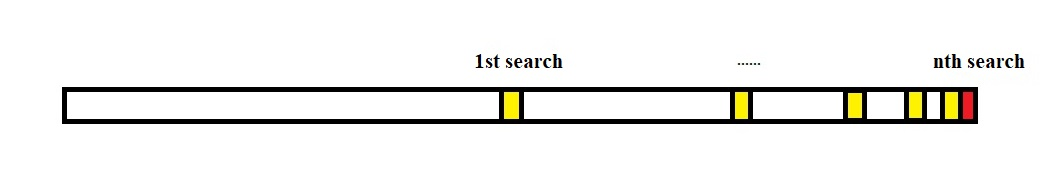
\includegraphics[width=\linewidth]{figs/I_2.jpg}
            \caption{Binary search, Yellow shows block, red shows last block}
            \label{fig:bs}
        \end{figure}
        
        \item ($2$ points)
        Consider the algorithm from the Course Notes that computes the average value in an $m\times m$ array~$A$ column by column, for the case where $A$ is stored in row-major order. In the Course Notes it was stated (on page~43) that the algorithm performs $n$~\ios, where $n := m^2$ is the total size of the array. The reason is that whenever we need a new entry from the array, we have already evicted the block containing that entry. This is true when the Least-Recently-Used replacement policy is used and when $m > M/B$, but it is not immediately clear what happens when some other replacement policy is used.
        
        Prove that when $m>2M/B$, then \emph{any} replacement policy will perform $\Omega(n)$~\ios.
        
        
        \item ($1+2\frac{1}{2}+2\frac{1}{2}$ points)
        Let $X[0..n-1]$ and $Y[0..n-1]$ be two arrays of $n$ numbers, where $n \gg M \gg B$. Suppose we have a function $f:\Reals^2\rightarrow \Reals$ and we want to compute $\min \{ f(X[i],Y[j]) : 0\leq i <n \mbox{ and } 0\leq j <n \}$. If we have no other information about $f$, then the only thing we can do is compute $f(X[i],Y[j])$ for all pairs $i,j$ with $0\leq i <n$ and $0\leq j <n \}$. A simple way to do this is using the following algorithm.
        %--------------------------------------------------------------------------------------------
        \begin{quotation}
            \noindent
            \emph{FindMin}$(X,Y)$ \\[-5mm]
            \begin{algorithmic}[1]
                \State $z \gets +\infty$
                \For{$i\gets 0$ \textbf{to} $n-1$}
                \For{$j\gets 0$ \textbf{to} $n-1$}
                \State $z \gets \min ( z, f(X[i],Y[j]) )$
                \EndFor
                \EndFor
                \State \Return $z$
            \end{algorithmic}
        \end{quotation}
        %--------------------------------------------------------------------------------------------
        \begin{enumerate}
            \item[(i)]
            Analyze the number of \ios performed by \emph{FindMin}.
            \item[(ii)]
            Give a cache-aware algorithm that solves the problem using $O(n^2/(MB))$ \ios, and prove that your algorithms achieves the desired \io-bound.
            
            \emph{Hint:} Partition both $X$ and $Y$ smaller subarrays, and solve the problem for each pair of subarrays separately.
            \item[(iii)]
            Give a cache-oblivious algorithm that solves the problem using $O(n^2/(MB))$ \ios, and prove that your algorithms achieves the desired \io-bound.
            
            \emph{Hint:} Use a recursive algorithm, and use a recurrence to analyze the \io-complexity. When writing the recurrence you should be precise about ``blocks sticking out'', similarly to what is done in the proof of Theorem~5.2. When solving the recurrence, you are allowed to ignore the blocks sticking out and work with a simplified recurrence.
        \end{enumerate}
        
        \textbf{Answer:}
        \begin{enumerate}
            \item[(i)]
            The algorithm contains two for loops, one outer loop, lines 2-6 of the algorithm, and one inner loop, lines 3-5 of the algorithm. All data of $X$ is read and compared linear, therefore $X$ has a $O(\frac{n}{B})$ \io complexity.
            
            Data from $Y$ is however read in the inner loop. Since $n \gg M$, this data has to be read for every cycle of the outer loop. The complexity of $Y$ is therefore $n \cdot O(\frac{n}{B}) = O(\frac{n^2}{B})$ \ios, which gives a total \io complexity of $O(\frac{n^2}{B})$ \ios.
            \item[(ii)]
            I designed the following algorithm:
            
            \emph{CacheAwareFindMin}$(X,Y)$
            \begin{algorithmic}[1]
                \State $t \gets B \cdot \lfloor M / B \rfloor$ - B
                \State $z \gets +\infty$
                \For{$i\gets 0$ \textbf{to} $n/t$}
                \State $X^* \gets X[i \cdot t : \min ((i+1) \cdot t - 1, n)]$
                \For{$j\gets 0$ \textbf{to} $n/t$}
                \State $Y^* \gets Y[j]$
                \State $z \gets \min (z, FindMin(X^*, Y^*))$
                \EndFor
                \EndFor
                \State \Return $z$
            \end{algorithmic}
            
            Instead of loading array entries one by one, we divide $X$ in bigger blocks that we load one by one in the internal memory. Lines 2-10 should be self-explaining. In order to minimize the \io complexity, we have to maximize $t = |X^*|$, so we get: $t = M$. To order with blocks sticking out, we divide by $B$, floor the result and then multiply by $B$ again. This way, we can take exact blocks from the external memory that will always fit into the internal memory. Since we need to reserve for one block of $Y$, we subtract $B$. 
            
            Again, the algorithm contains two for loops. All data of $X$ is linear read in the outer loop exactly one time, so we have again an \io complexity of $O(\frac{n}{B})$ \ios for $X$. The inner loop has again the same problem as before: since $n \gg M$, $Y$ has to be read once time for every cycle of the outer loop. This gives an \io complexity of $\frac{n}{t} \cdot O(\frac{n}{B}) = \frac{n}{B \cdot \lfloor M / B \rfloor - B} \cdot O(\frac{n}{B}) < \frac{n}{M} \cdot O(\frac{n}{B}) = O(\frac{n^2}{MB})$ \ios.
            \item[(iii)]
            I designed the following algorithm:
            
            \emph{CacheObliviousFindMin}$(X, i_1, i_2, Y)$
            \begin{algorithmic}[1]
                \If{$i_1 = i_2$}
                \State $z \gets +\infty$
                \For{$j\gets 0$ \textbf{to} $n-1$}
                \State $z \gets \min (z, f(X[i_1],Y[j]) )$
                \EndFor
                \Else
                \State $i_{mid} \gets \lfloor (i_1 + i_2) / 2 \rfloor$
                \State $z_1 \gets CacheObliviousFindMin(X, i_1, i_{mid}, Y)$
                \State $z_2 \gets CacheObliviousFindMin(X, i_{mid} + 1, i_2, Y)$
                \State $z \gets \min (z_1, z_2)$
                \EndIf
                \State \Return $z$
            \end{algorithmic}
            
            One way to think about \emph{CacheObliviousFindMin} is that it recursively partitions $X$ into sub-arrays until the sub-arrays are such that they fit into the memory next to one block of $Y$, in other words, the size of a sub-array is smaller than or equal to $M-B$. In such a situation, we have an \io complexity of $O(\frac{n}{B})$ because of array $Y$. The question now is: how many of these situations are recursively created? In the best case scenario, we have $\frac{n}{M-B}$ of these situations. In the worst case, we have no more than $2 \cdot \frac{n}{M-B}$ of these situations. So our total \io complexity becomes $2 \cdot \frac{n}{M-B} \cdot O(\frac{n}{B}) < 2 \cdot \frac{n}{M} \cdot O(\frac{n}{B}) = O(\frac{2 \cdot n^2}{MB}) = O(\frac{n^2}{MB})$ \ios.
        \end{enumerate}
        
    \end{rlist}
    
    %------------------------------------------------------------------------------
    \renewcommand{\setnr}{IO.II}
    \subsection*{Exercise Set I/O-Efficient II}
    %------------------------------------------------------------------------------
    \begin{rlist}
        
        \item (2 points)
        Consider an algorithm that needs at most $c n\sqrt{n} / (MB)$ \ios if run with
        optimal caching, for some constant $c$. Prove that the algorithm needs at most
        $c' n\sqrt{n} / (MB)$ \ios when run with \lru caching, for a suitable constant $c'$.
        \\[2mm]
        \emph{Hint:} Compare the performance of both versions to running the algorithm with optimal
        caching on a machine that has only half as much memory.
        
        \item ($1$ point)
        Suppose we wish to sort a set of $n$ numbers.
        For the special case where the input consists of integers in the range $1,\ldots,n^2$,
        there exists a sorting algorithms that runs in $O(n)$ time.
        Is it possible that this algorithm performs $O(n/B)$ \ios for
        any input of size~$n$? Briefly explain your answer.
        
        
        
        \item (3 points)
        Analyze the running time (not the number of \ios) of algorithm \emph{EM-MergeSort}.
        Does it still run in $O(n\log n)$ time? If not, explain how to implement the
        merge step to make it run in $O(n\log n)$ time.
        
        
        \item(3 points)
        In the proof of Theorem~6.2 we assumed that the algorithm only
        uses the blocks of the input array $A$, it does not use any additional storage
        in the external memory. Prove that without this assumption the same asymptotic lower
        bound holds.
        \\[2mm]
        \emph{Hint:} Consider a permutation algorithm that \emph{does} use additional memory blocks.
        Show that the algorithm can be modified such that the assumption is satisfied---that is,
        such that all write operations are to blocks in $A$---while not increasing the number
        of \ios by more than a factor~3.
    \end{rlist}
    
    
    
    
    %------------------------------------------------------------------------------
    \renewcommand{\setnr}{IO.III}
    \subsection*{Exercise Set I/O-Efficient III}
    %------------------------------------------------------------------------------
    
    \begin{rlist}
        
        \item ($2 + 2$ points)
        Consider a balanced binary search tree $\tree$ with $n$ internal nodes that is stored in external memory.
        You may assume that $n=2^k-1$ for some integer~$k$, and that the tree is perfectly balanced.
        Hence, its depth is~$\log_2 (n+1)$.
        \begin{enumerate}
            \item[(i)]
            Describe blocking strategy that guarantees that any root-to-leaf
            path in $\tree$ can be traversed in $O(\log_B n)$. What is the relation of your blocking
            strategy to B-trees?
            \item[(ii)]
            Prove that for \emph{any} blocking strategy there will be a root-to-leaf path that
            visits $\Omega(\log_B n)$ blocks. To simplify the proof you may assume that
            the blocking strategy has the following property: for each block $b$, the nodes in
            $b$ form a connected part of $\tree$. This implies that whenever a root-to-leaf path
            leaves a block, it will not re-enter that block. 
        \end{enumerate}
        
        \item (2 points)
        The \io-efficient priority queue described above keeps a set $S^*$ in internal memory
        that contains $M/4$ elements when $S^*$ is created. The next $M/4$ operations are then
        performed on $S^*$, after which the elements that still remain in $S^*$ are inserted
        into the buffer tree (and $S^*$ is emptied).
        Someone suggests the following alternative approach: instead of only performing
        the next $M/4$ operations on $S^*$, we keep on performing
        \emph{Extract-Min} and \emph{Insert} operations on $S^*$ until $|S^*|=M$.
        Does this lead to correct results? Explain your answer.
        
        \item (4 points)
        A \emph{coloring} of an undirected graph~$\G=(V,E)$ is an assignment of colors to
        the nodes of $\G$ such that if $(v_i,v_j)\in E$ then $v_i$ and $v_j$ have different colors.
        Suppose that $\G$ is stored in the form of an adjacency list in external memory.
        Assume the maximum degree of any node in $\G$ is~$d_{\max}$. Give an algorithm that computes
        a valid coloring for $\G$ that uses at most $d_{\max}+1$ colors. Your algorithm should perform
        $O(\sort(|V|+|E|)$ \ios.
        
    \end{rlist}
    
\end{document} 

